\documentclass[11pt,onecolumn,letterpaper]{article}
\usepackage[margin=2.5cm]{geometry}
\usepackage{times,epsfig,graphicx,amsmath,amssymb,cite}
\usepackage{multirow}
\usepackage{booktabs}
\usepackage{tabularx}
\usepackage[breaklinks=true,colorlinks=true,bookmarks=false]{hyperref}
\date{}

%%%%%%%%%%%%%%%%

\title{Improved Metric Learning Method Implemented in Classification Task}

\author{%
Xiaochen Zhou, Jiahao Li, Xiwen Li\\
{\tt zhouxiaochen@wustl.edu, xx@wustl.edu, xx@wustl.edu}
}


\begin{document}
\maketitle

\begin{center}\textbf{Abstract}\\~\\\parbox{0.85\textwidth}{\em
    % Abstract goes here

As a powerful method for recognition and re-identification task, metric learning greatly improve the accuracy and performance of tasks which require distance optimization between different features. Taking this property into consideration, we come out with the method to optimize the classification method with triplet loss method and improve this method to better suit the requirement of classification task. We will implement the method with convolutional neural network and make the comparison of the performance of classification between original CNN, CNN with triplet loss and CNN with our improved triplet loss.
}\end{center}

\section{Introduction}

Metric learning, highly related to similarity learning, is an area of supervised machine learning in artificial intelligence. As a powerful method to learn from examples a similarity function that measures how similar or related two objects are, metirc learning is widely use in tasks like face recognition and re-identification tasks, where the difference between special sections are much more important than the distance of the global features. Compared with classification tasks, datasets for these tasks share high similarity and the global feature supervised by softmax-entropy loss is not strong enough to clarify the difference between two faces. Metric learning method, like triplet loss which is used in this paper, is invented for further optimization. By enlarging the distance between classes, called intra-class distance and lowering the distance in the same classes, called inter-class distance, metric learning make it possible for the machine learning model to tell the difference between two similar objects.

Considering the property of metric learning, some supervising signal like triplet loss can be exerted in model training as the auxiliary loss. This method will improve the performance of classification for neural network, especially for some hardcore classification task, like sofa and chair, sofa and bed etc., which shares relatively higher similarity. Also, the auxiliary loss can cluster the classes much tighter, to some extent avoiding overfitting for the small dataset.

In this paper, we optimize triplet loss as a new supervising signal, semi-hardcore triplet loss, to help improve the performance of classification task with the assistance of convolutional neural network (CNN). Several researchers paid attention to the improvement of softmax-entropy loss function and intra-class distance optimization. Lee et.al \cite{lee2018dropmax} takes the advantages of dropout method to lower the inter-class distance. Deli{\'e}ge et.al \cite{deliege2018hitnet} developed a new hit-and-miss layer for the better performance of softmax-entropy loss. Useful as these method, new layers implemented in neural network increases the computation complexity and makes the training process longer. Using metric learning method as auxiliary loss function, however, effectively avoid the increasing computation and improve the classification performance at the same time, making the neural network training more efficient. Then, our method will improve the capability for the loss to tighten the inter-class distance and enlarge the intra-class distance.

To implement the optimization signal, we conduct two experiment with the assistance of semi-hardcore triplet loss. First, we work on the classification task with softmax-entropy loss with triplet loss on dataset Caltech 101\cite{griffin2007caltech} to test the performance of classification job. 102 classes are contained in this dataset, 80 to 200 images for each class. In dataset, we get the classes with similar features and properties, such as corcodile class and crocodile-head class, which fits our requirement to test the capability of classifying classes with close distance. Second, we recurrent a 3D model recognition task with score mapping, called View Discerning Network \cite{leng2018learning}, to evaluate the classification of 3D models from 2D projected images. Considering that projections from different classes may be very similar, where the side projection of a door is close to the projection of a wood stick, the score mapping for these projection may be the same. However, the side projection of the door only contains little useful attributes and features for the recognition of 3D models, which is called bad view, and, in the opposite, the side projection for a wood stick should be evaluated as good view owing that the shape of wood stick is just like a bonded line. In this case, good views and bad views may be judged as the same contribution to the recognition. We will recurrent this method and implement triplet loss on this method to help improve the performance of the score mapping network.

An overview of the following sections are as follow: In section 2 we will introduce the related work on metric learning. In section 3, algorithms for our method will be given and analyzed. Then section 4 will show the performance of classification among bared softmax-entropy loss, loss with triplet loss and loss with improved triplet loss. Last section will be the conclusion.


\section{Background \& Related Work}

\begin{figure}[t]
\centering
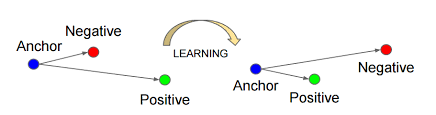
\includegraphics[width = 0.8\textwidth]{triplet.png}
\label{triplet}
\caption{Vistualization of triplet loss function}
\end{figure}

Metric learning is an area of deep learning. Even though it is related to regression and classification, its goal is to example a similarity function that measure how similar two objects are. As one example of metric learning, triple loss is widely used in research on person re-identification problems, especially re-identifying persons. Models based on classification, siamese network and triplet models are three popular method of dealing with person re-identification problem. Loss functions used are categorized into pairwise loss function and triplet loss function. Euclidean distance is a common used metric of triplet loss function. 
\newline
We are going to introduce several research examples taking advantages of deep learning in which good results are obtained. Hao Liu \cite{liu2016end} combines triplets loss and identification loss to train a end-to-end comparative attention networks. The loss function of ours is similar with theirs. Chi Su \cite{su2016deep} proposes a semi-supervised attribute learning model with three stages and embed triplet loss in the second stage. Rahul Rama Varior \cite{varior2016learning} uses regular loss function to train a CNN model. Wang \cite{wang2014learning} uses triplet training examples and the triplet loss function to learn fine grained image to similarity metrics. They built a deep ranking model that employs a novel and efficient triplet sampling algorithm. Their output outperforms common models. With regards to human faces and human appearance, FaceNet \cite{schroff2015facenet} uses triplets of aligned matching / non-matching face patches when training. Their method both improve the efficiency and the performance. On one hand, their representational data only needs 128-bytes per face. On the other hand, their model achieves new record accuracy of 99.63\% and 95.12\% on YouTube Faces DB. Ejaz Ahmed \cite{ahmed2015improved} build a deep neural network model that trains the similarity between two parallel input pictures pair-wisely. Their model includes a layer that computes pixel wise difference between input images and a patch summary layer to get high-level features. Similarly, Yi et al. \cite{yi2014deep} constructs a Siamese neural network to learn pair-wise similarity between bodies. They crop each human body into three parts, train separately and fuse when calculating loss. Following them, Cheng et.al \cite{cheng2016person} borrows their idea and built their own multi-channel CNN. They modify the regular CNN by substituting regular loss function with triplet loss in order to pull the loss difference between pictures of the same person closer, while pulling it between pictures of different persons bigger. Their work is divided into feature extraction and distance metric for comparing features across images. Their network constructs multi-layer deep neural network in order to capture and to train both global and local features of human bodies. Also, their triplet loss function enables features from the same person closer and different persons further away. Based on regular $L_{2}$-norm distance, their triplet loss function is the summation between mean of inter-class constraint and intra-class-constraint. By applying their model on four different popular person re-identification benchmark datasets, they achieve higher accuracy than other previous researchers.

\section{Algorithm}
\subsection{Triplet Loss and Semi-hardcore Triplet Loss}
Triplet loss is first invented in Scgriff et.al \cite{schroff2015facenet}, which is exerted in face recognition task. The embedding system of triplet loss is functioning as follows. An image is set as the input of the neural network and the feature is extracted in a $d$-dimensional Euclidean space. To improve the performance of face recognition, another two images are sent into network as a triplet pair, where the original input is called image $x_i^a$ (anchor), the image sharing the same class with anchor image $x_i^p$ (positive) and the image with different class with anchor image $x_i^n$ (negative). To enlarge the inter-class distance and lower the intra-class distance, the equation can be written as follows:
$$||x_i^a - x_i^p||_2^2 + \alpha < ||x_i^a - x_i^n||_2^2, (x_i^a, x_i^p, x_i^n) \in \Gamma$$

where $\alpha$ is the margin distance between positive pairs and negtive pairs and $\Gamma$ is the set of all possible triplet pairs $N$ in training period. Figure \ref{triplet} visualize the process of optimization for triplet loss. Then the loss function can be expressed as follows:
$$Loss = \sum_{i}^N [||x_i^a - x_i^p||_2^2  - ||x_i^a - x_i^n||_2^2 - \alpha]_+$$

Then to improve the performance of classification, we need to do some changes on data selection. Owing to the differences for recognition tasks are relatively small, using metric learning can making the training period unconverging. However,  considering that the difference between class in classification task is usually larger than recognition tasks, we do not need to worry too much about the negtive influence from dataset. On contrast, we need to modify the loss function, making to stronger for classification tasks.

For training period, when anchor image is set, we search the dataset to find an image  with the largest distance in the same class and to find an image with the lowest distance in different classes. The equation can be written as follows:

$$Loss = \min_{x_i^p}\max_{x_i^n} \sum_{i}^N [||x_i^a - x_i^p||_2^2  - ||x_i^a - x_i^n||_2^2 - \alpha]_+$$

\begin{figure}
\centering
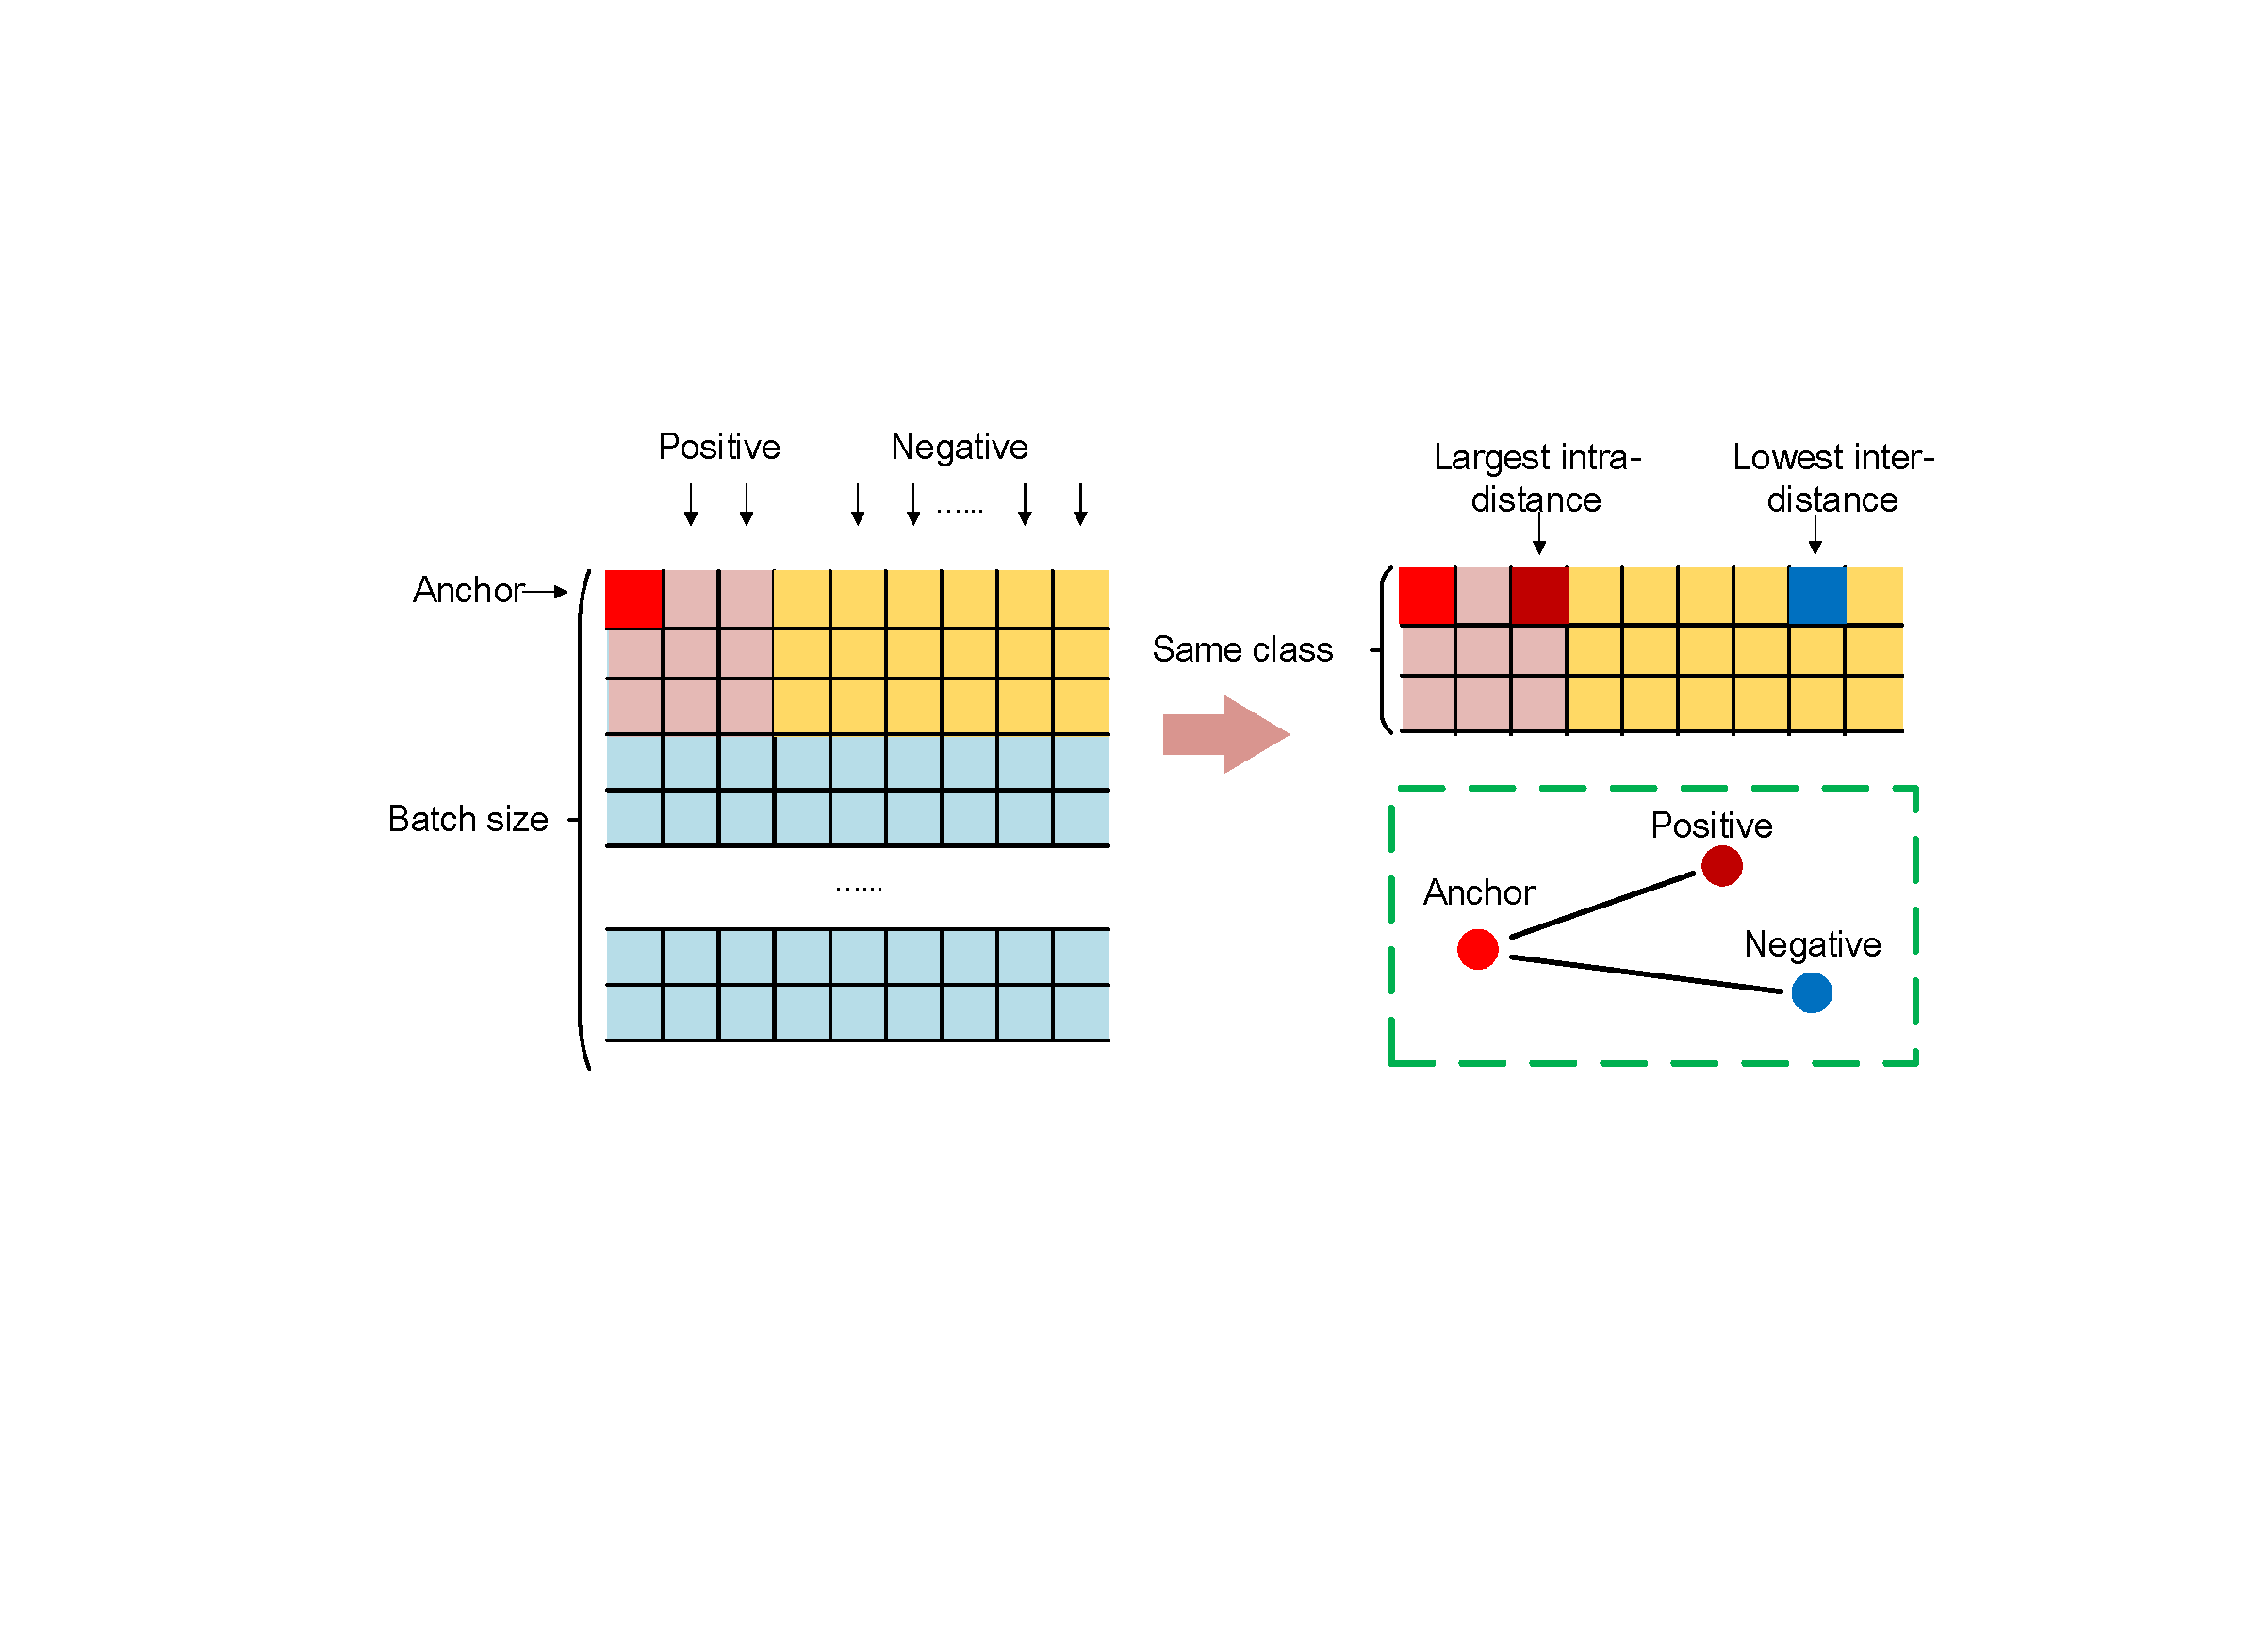
\includegraphics[width = 0.8\textwidth]{improve.pdf}
\label{improved}
\caption{Vistualization of semi-hardcore data selection for triplet loss function}
\end{figure}

This method make the loss function more hardcore than the function for recognition. However, searching for the largest distance for positive image and lowest distance for negative image is time-consuming, especially when the dataset is large. To optimize the data selection, instead of search for the whole dataset, a semi-hardcore method is implemented in this method. Considering our method is use in neural network, each time we send data into the network, we cluster the data via classes, which means, images in the same class will be gathered together. In this case, we can calculate the distance for each two images in one batch, then rank the distance to achieve the best selection in one batch. Figure \ref{improved} clarifies the process of optimization.

\subsection{3D Model Recognition}

\begin{figure}[htbp]
\centering
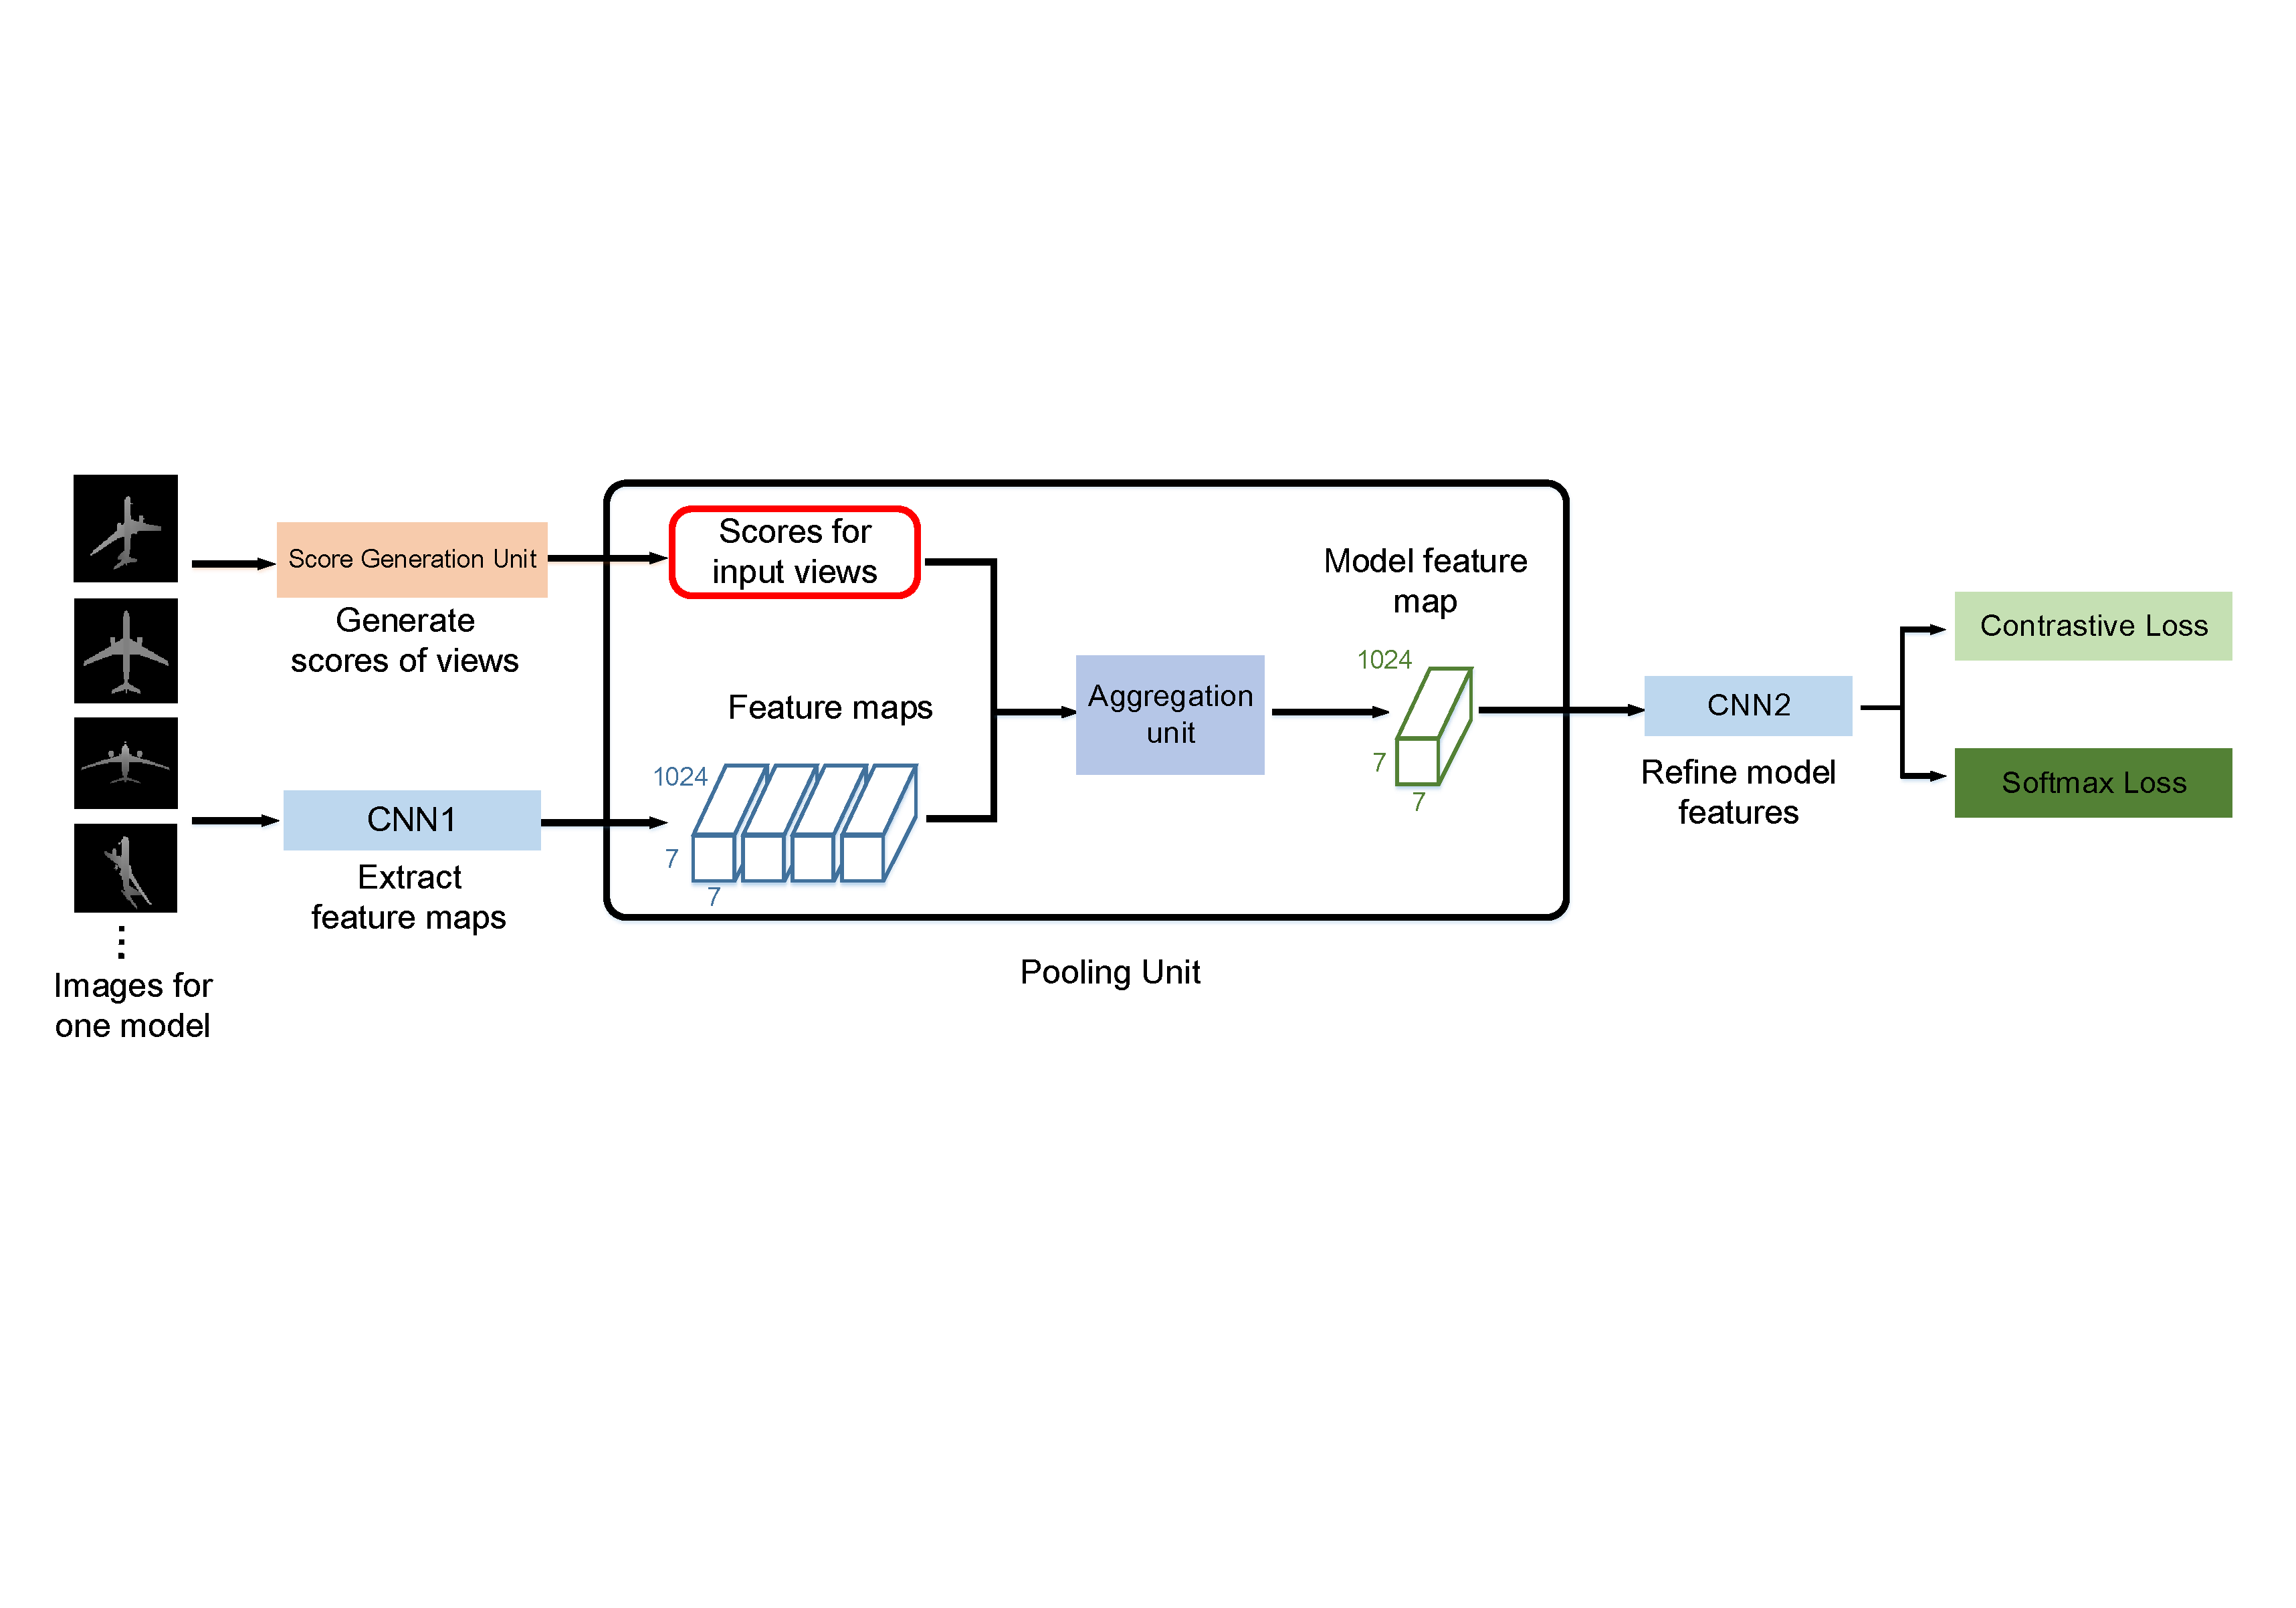
\includegraphics[width = 0.8\textwidth]{procedurepic.pdf}
\label{3d}
\caption{The structure of View Discerning Network}
\end{figure}

\begin{figure}[htbp]
\centering
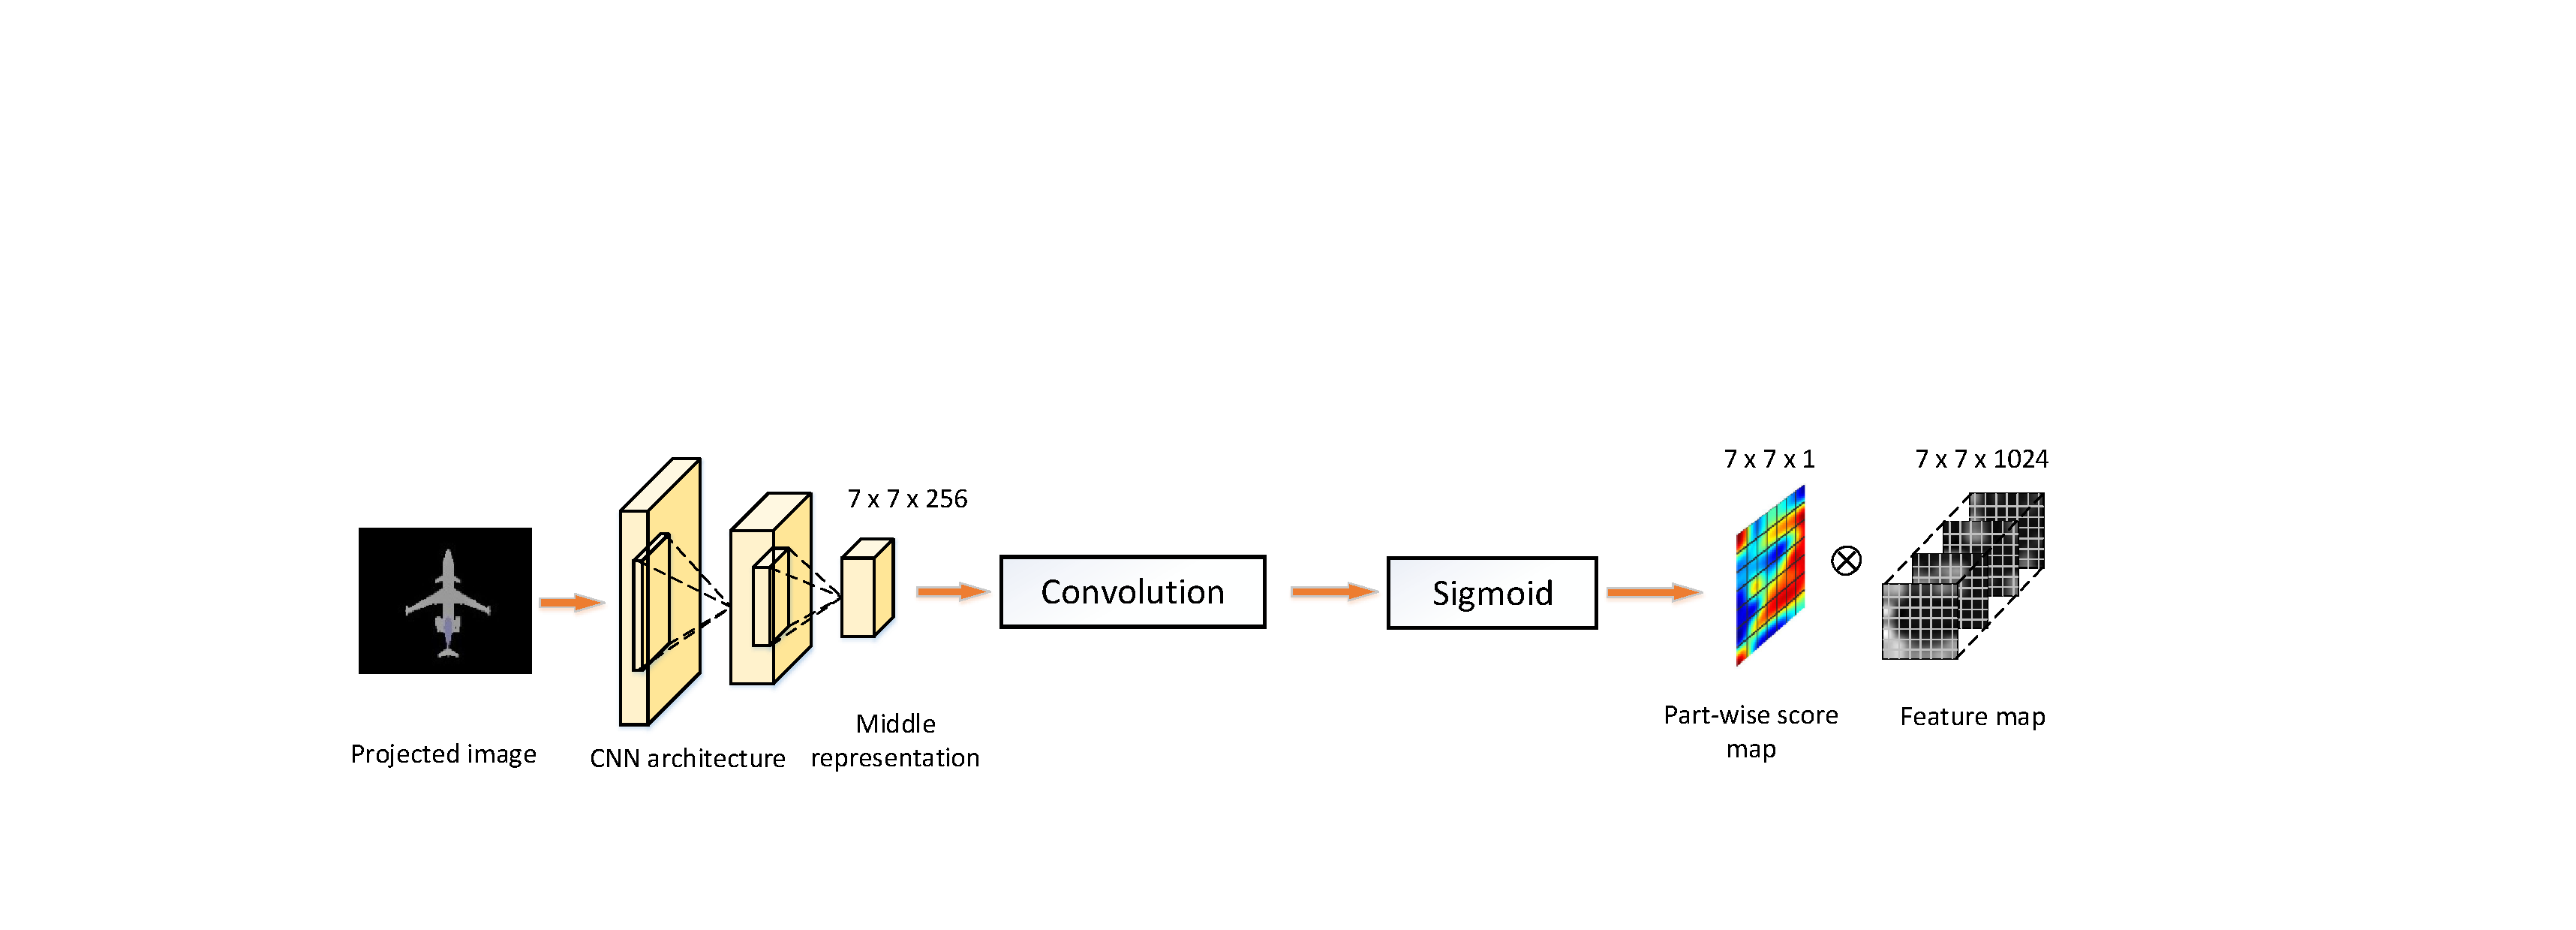
\includegraphics[width = 0.8\textwidth]{scorePic.pdf}
\label{score}
\caption{The structure of Part-wise Score Unit}
\end{figure}
To evaluate the performance of recognition between projection features with high similarity, we implement the triplet loss to a 3D model recognition model, called View Discerning Network (VDN). Figure \ref{3d} shows the stucture of the network.

VDN is utilized to approach the quality of views and aggregate their features based on the evaluation scores. Specifically, a branch network, Score Generation Unit (SGU), is introduced to the standard CNN to evaluate the quality of each projected image with score vectors. These score vectors are then used to weigh the image features and their summation serves as the representation of the shape. The weighted features are further refined by CNN.

For the structure of Score Generation Unit, two structures focusing on different aspects of image features are introduced. The first structure is called Channel-wise Score Unit, where channels correspond to filters of the CNN. And each filter produces a feature map for the image. For every channel, Channel-wise Score Unit generates a certain score which is applied to the feature map. Consequently, this structure emphasizes the difference of feature maps extracted by different filters. The second structure, named Part-wise Score Unit, concentrates on the difference of local region of the image. It measures each part of the feature map based on the regional information, yielding a score map with the same size of the feature map. And the feature maps from the same image all share the same score map. For the better visualization result, we use the Part-wise Score Unit as the score mapping unit and we believe that the optimization for scores generated by Part-wise Score Unit.

According to the network, a supervision signal called Contrastive loss is used as an auxiliary signal to improve the performance the recognition. With these supervision signals, views with high quality become dominant among others, since they are assigned with higher scores. In our experiment, we remove this signal, using the triplet loss and improved triplet loss instead. Also, we use the average merge method as the comparison. We will judge the performance of score mapping, which is shown in the next section.


\section{Experimental Results}

\subsection{Dataset}
\subsubsection{Caltech 101}
In the experiment, we implement the neural network in Caltech 101 dataset \cite{griffin2007caltech}. The number of classes is 101, about 40 to 800 images per category. Most categories have about 50 images. Collection was finished in September 2003 by Fei-Fei Li, Marco Andreetto, and Marc 'Aurelio Ranzato. The size of each image is roughly 300 x 200 pixels. For training period, 70\% of images in one class are selected as training set and 30\% of images are picked as testing set. For the baseline, we select several models like Alexnet, for classification task. We extract features from the last dropout layer and send it to both fully-connection layer for softmax-entropy loss, triplet loss and semi-hardcore triplet loss as supervising signal.

\subsubsection{ModelNet}
This dataset is composed of 662 categories with 127,915 shapes from daily life. The core of the dataset is compiled to a list of the most common object categories in the world. ModelNet includes two subsets, ModelNet 40 and ModelNet 10. ModelNet 40 contains 12,311 shapes from 40 categories and ModelNet 10 possesses 4,899 shapes from 10 categories, both of which are utilized in our experiment. For these two datasets, we randomly choose at most 80 shapes from every category for training and 20 shapes for testing.

\subsubsection{ShapeNet Core55}
This dataset is introduced in SHape recognition Contest (SHREC), which concentrates on the scalability of 3D shape recognition methods. Hence, we exert this large-scale dataset in our experiment, which contains about 51,190 3D shapes from 55 common categories, each subdivided into 204 subcategories. This dataset is divided into two parts, normal dataset and perturbed dataset. shapes in normal datasets are all aligned in one direction and shapes in perturbed datasets are randomly rotated. All the shapes are divided into three parts, 70\% used for training, 10\% for validation and 20\% for testing.  To test the robustness of View Discerning Network, we adopt both normal datasets and perturbed datasets for the experiment. In ShapeNet Core55 datasets, we adopt MAP, F-measure, and NCDG as the standard of the judgment. Besides, Precision-Recall Curves are used to intuitionally show the comparison between View Discerning Network and other methods on the State-of-the-Art.

\subsection{Data organization \& Experimental Setup}

Caltech 101 dataset totally has approximately 9000 pictures. About 30\% pictures are randomly selected from each categories as our testing data set. Test data is evenly chosen from all classes. The rest of images are for training. We use stochastic gradient decent to train the dataset. Their sizes are rescaled in order to feed into our network. Two batch generators are built for our baseline and Improved loss function. For each batch, we implement special customized data structure to meet the form of our triplet loss function. The baseline generator aligns three-picture group. The front two belong to the same categories, while the last picture belongs to another class. The improved generator divides pictures into classes and put images from the same class together.

As for the experimental setup, we adopt the 50-layer version of ResNet as our neural network model. Since the Caltech 101 dataset is relatively small, we first train the network on the large ImageNet dataset, and then fine-tune it on the Caltech dataset. The optimization method is stochastic gradient descent (SGD) with momentum. The learning rate is set to 0.001 and momentum set to 0.9. The network is fine-tuned on a single Nvidia GTX 1080Ti GPU for 5 epochs.
\subsection{Results \& Comparison}

\subsubsection{Classification Task}
\begin{table}[htbp]
\renewcommand{\arraystretch}{1.3}
\centering
\caption{Comparision of Convergence Speed}
\label{speed}
\resizebox{0.8\textwidth}{13mm}{
\begin{tabular}{lcccccc}
\hline
Epoch&1&2&3&4&5\cr
\hline
Baseline&74.72\%&88.62\%&91.82\%&92.45\%&93.33\%\cr
Triplet\_loss&78.43\%&89.25\%&91.19\%&93.71\%&94.03\%\cr
Improved\_Triplet\_loss&79.94\%&90.40\%&92.57\%&94.24\%&95.03\%\cr
\hline
\end{tabular}}
\end{table}
Table \ref{speed} shows the test accuracies of training the network with cross entropy loss and triplet loss respectively. At the end of the first epoch, the test accuracy of triplet loss is higher than that of the cross entropy loss by 3.71\%. This shows that triplet loss enables faster convergence than cross entropy loss. Also, the eventual performance of the triplet loss is superior to that of the cross entropy loss.
We also carry out experiments to show the effect of the hyper-parameter $\alpha$ and $\lambda$. The results are summarized in figure xx and figure yy. It can be seen that ...

\subsubsection{3D Model Recognition}

In this section, we will illustrate the results in 3D model recognition task. To compare the performance of recognition, in each experiment, we train the VDN congregated with max pooling score mapping and average pooling score mapping as baseline. Then we will train VDN with Part-wise Score Unit supervised by triplet loss and semi-hardcore triplet loss and make comparison. Here we call the semi-hardcore triplet loss as improved triplet loss for convenience. 

First, the experiment is implemented on ModelNet dataset, where both ModelNet 40 and ModelNet 10 are used. The result can be found in Table \ref{modelnet}. As can be seen, VDN with PSU is much better than baseline, which has been proved in \cite{leng2018learning}. Then, VDN supervised by triplet loss and improved triplet loss obtain better performance than normal VDN and improved triplet loss is show stronger recognition capability, where improved triplet loss VDN is around 1.5\% higher than VDN with normal triplet loss in each criteria.

\begin{table}[!htbp]
\renewcommand{\arraystretch}{1.3}
\centering
\caption{Performance comparision of 3D shape recognition on ModelNet datasets}
\label{modelnet}
\begin{tabular}{lcccc}
\hline
\multirow{2}{*}{Method}&
\multicolumn{2}{c}{ModelNet 40}&\multicolumn{2}{c}{ModelNet 10}\cr
\cmidrule(lr){2-3} \cmidrule(lr){4-5}
&AUC&MAP &AUC&MAP\cr
\hline
VDN\_MAX&83.14\%&81.90\%&91.75\%&91.31\%\cr
VDN\_AVE&83.07\%&81.85\%&91.66\%&91.23\%\cr
VDN\_Triplet&86.33\%&84.92\%&91.10\%&9.34\%\cr
VDN\_Improved\_Triplet&87.62\%&86.64\%&93.15\%&92.80\%\cr
\hline
\end{tabular}
\end{table}

Then for the next dataset SHREC, we use the same strategy for the experiment on this dataset. The result can be found in Table \ref{SHREC_normal} and Table \ref{SHREC_perturbed}. In the experiment on SHREC, three new parameters are adopted, Macro-version (Macro), Micro-version (Micro) and mean of Macro-version and Micro-version (Macro+Micro), to judge the capability of the method. Macro offers an unweighted average for the whole datasets, while Micro is used to adjust the shape category sizes via considering a representative performance across categories. As for normalized discounted cumulative gain (NDCG), NDCG metric uses a graded relevance: 3 for perfect category and subcategory match in query and retrieval, 2 for category and subcategory both being same as the category, 1 for correct category and a sibling subcategory, and 0 for no match.

\begin{table*}[!htbp]
\renewcommand{\arraystretch}{1.3}
\centering
\caption{Performance comparision of 3D shape recognition on ShapeNet Core55 normal datasets}
\label{SHREC_normal}
\resizebox{\textwidth}{17mm}{
\begin{tabular}{lccccccccc}
\hline
\multirow{2}{*}{Method}&
\multicolumn{3}{c}{Micro}&\multicolumn{3}{c}{Macro}&\multicolumn{3}{c}{Micro + Macro}\cr
\cmidrule(lr){2-10}
&F-measure&MAP&NCDG&F-measure&MAP&NCDG&F-measure&MAP&NCDG\cr
\hline
VDN\_MAX&0.674&0.797&0.824&0.485&0.732&0.804&0.580&0.765&0.814\cr
VDN\_AVE&0.689&0.825&0.896&0.454&0.740&0.850&0.572&0.783&0.873\cr
\hline
VDN\_Triplet&0.766&0.892&0.913&0.578&0.831&0.899&0.672&0.862&0.906\cr
VDN\_Improved\_Triplet&0.791&0.911&0.943&0.599&0.857&0.914&0.695&0.884&0.929\cr
\hline
\end{tabular}}
\end{table*}

\begin{table*}[!htbp]
\renewcommand{\arraystretch}{1.3}
\centering
\caption{Performance comparision of 3D shape recognition on ShapeNet Core55 perturbed datasets}
\label{SHREC_perturbed}
\resizebox{\textwidth}{17mm}{
\begin{tabular}{lccccccccc}
\hline
\multirow{2}{*}{Method}&
\multicolumn{3}{c}{Micro}&\multicolumn{3}{c}{Macro}&\multicolumn{3}{c}{Micro + Macro}\cr
\cmidrule(lr){2-10}
&F-measure&MAP&NCDG&F-measure&MAP&NCDG&F-measure&MAP&NCDG\cr
\hline
VDN\_MAX&0.612&0.734&0.843&0.416&0.662&0.793&0.514&0.698&0.818\cr
VDN\_AVE&0.594&0.749&0.865&0.382&0.579&0.767&0.488&0.664&0.816\cr
\hline
VDN\_Triplet&0.668&0.831&0.890&0.430&0.735&0.844&0.549&0.783&0.867\cr
VDN\_Improved\_Triplet&0.686&0.843&0.897&0.442&0.751&0.858&0.564&0.797&0.878\cr
\hline
\end{tabular}}
\end{table*}

As can be seen from tables that in each dataset, VDN supervised by triplet loss and improved triplet loss perform better, and improved triplet loss is also stronger than normal triplet loss. 

In conclusion, all the experiments above prove that metric learning in classification task and recognition task can help improve the performance, and the semi-hardcore triplet loss can in advance benefit the tasks.

\section{Conclusion}
We exert a classic metric learning method, triplet loss, into classification task and 3D model recognition task and do some optimzations specially for these two tasks. Owing to the property of classification and neural network training, semi-hardcore model for data selection is used for this task. The performance of triplet loss and semi-hardcore triplet loss is better than normal training in training speed and accuracy, which prove that metric learning can improve the performance of some tasks which requires to lower the intra-class distance and higher the intro-class distance.


{\small
\bibliographystyle{ieee}
\bibliography{refs} % Create file refs.bib, and run bibtex.
}

\end{document}
